\documentclass{article}
\usepackage{tikz}
\usetikzlibrary{decorations.markings}
\pagestyle{empty}
\begin{document}
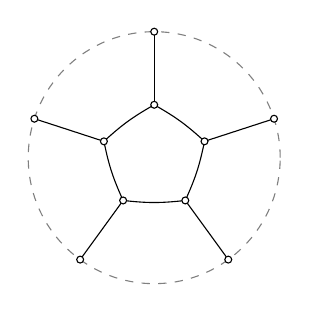
\begin{tikzpicture}
[scale=1.6,every node/.style={draw, circle, fill=white, inner sep=0pt, outer sep=0pt, minimum size=2.5pt},
->-/.style={decoration={markings, mark=at position .5 with{\arrow{>}}}, postaction={decorate}},
-<-/.style={decoration={markings, mark=at position .5 with{\arrow{<}}}, postaction={decorate}}]
\draw[gray, dashed] (0,0) circle (1.0);
 \node (6) at (0.0,1.0) {};
\node (7) at (-0.951057,0.309017) {};
\node (8) at (-0.587785,-0.809017) {};
\node (9) at (0.587785,-0.809017) {};
\node (10) at (0.951057,0.309017) {};
\node (1) at (0.3993,0.1297) {};
\node (2) at (-0.0,0.4198) {};
\node (3) at (0.2468,-0.3396) {};
\node (4) at (-0.2468,-0.3396) {};
\node (5) at (-0.3993,0.1297) {};
\draw[out=-162.000008, in=18.0] (10) to (1);
\draw[out=125.999988, in=306.0] (9) to (3);
\draw[out=54.000012, in=234.0] (8) to (4);
\draw[out=-17.999992, in=162.0] (7) to (5);
\draw[out=-90.0, in=90.0] (6) to (2);
\draw[out=138.0, in=330.0] (1) to (2);
\draw[out=258.0, in=426.0] (1) to (3);
\draw[out=546.0, in=354.0] (3) to (4);
\draw[out=474.0, in=282.0] (4) to (5);
\draw[out=210.0, in=402.0] (2) to (5);
\end{tikzpicture}
\end{document}